\chapter{Identification and tuning of the controllers}\label{ch:tuning}
In this chapter we will look at the tuning of the different controllers of the system. Firstly we will look at the secondary controllers, before we later move on to the higher level controlllers. A summary of the different controller parameters can be found in \autoref{table:controllerparam}.

\begin{table}[h]
	\caption{Summary of controller parameters in the plant}
	\label{table:controllerparam}
	\begin{center}
	\begin{tabular}{|c|c|c|c|}
	\hline
	Controller & $K_p$ & $T_i$ & $T_d$ \\
	\hline
	\texttt{24\_FC1005} & $1.18125$ & $5$ & - \\
	\texttt{24\_FC1015} & $0.2$ & $5$ & -\\
	\texttt{24\_FC1019} & $0.27225$ & $5$ & - \\
	\texttt{24\_LC1028} & $47.9$ & $128$ & - \\
	\texttt{24\_PC1024} & $17.5$ & $2400$ & -
	\end{tabular}
	\end{center}
\end{table}

\section{Tuning of secondary controllers}\label{sec:tuning_secondary}
Firstly we want to tune the secondary controllers, which do not depend much on which control structure is used for composition control. The controllers this applies to is the flow controllers \texttt{24\_FC1005}, \texttt{24\_FC1015} and \texttt{24\_FC1019}, the level controller \texttt{24\_LC1028}, and also the pressure controller \texttt{24\_PC1024}. These controllers all have fast dynamics compared to the composition control and primary level controllers.

\subsection{Tuning of \texttt{24\_FC1019}}
Firstly we tune the controller \texttt{24\_FC1019}, which is a flow controller controlling the bottom flow $B$ of N-butane. When trying to apply Skogestad IMC-tuning to a first order model, the results were poor as there are close to none time delay, as expected in a valve, which lead to this being a unprecise model. Ziegler-Nichols method, as described in \cite{balchen2003reguleringsteknikk}, was then a natural choice, and with a critical gain of $K_{p_k} = 0.605$ and integral time $T_i \to\infty$ we got the osciallations shown in \autoref{fig:fc1019_oscillations}. By zooming into this we read the period of the oscillations as $T_k = \SI{6}{\second}$. This yields the gain and integral time $K_p = 0.27225$ and $T_i = \SI{5}{\second}$. With this tuning we get the response shown in \autoref{fig:fc1019_tuned}. This is a good response to a relatively large step reference change. Before the reference step the controller has an external set point, that is why the set point is changing dynamically. When doing the step change, the controller settings was changed from external to internal set point, and then back to external for the second step.

\begin{figure}[ht!]
	\centering
	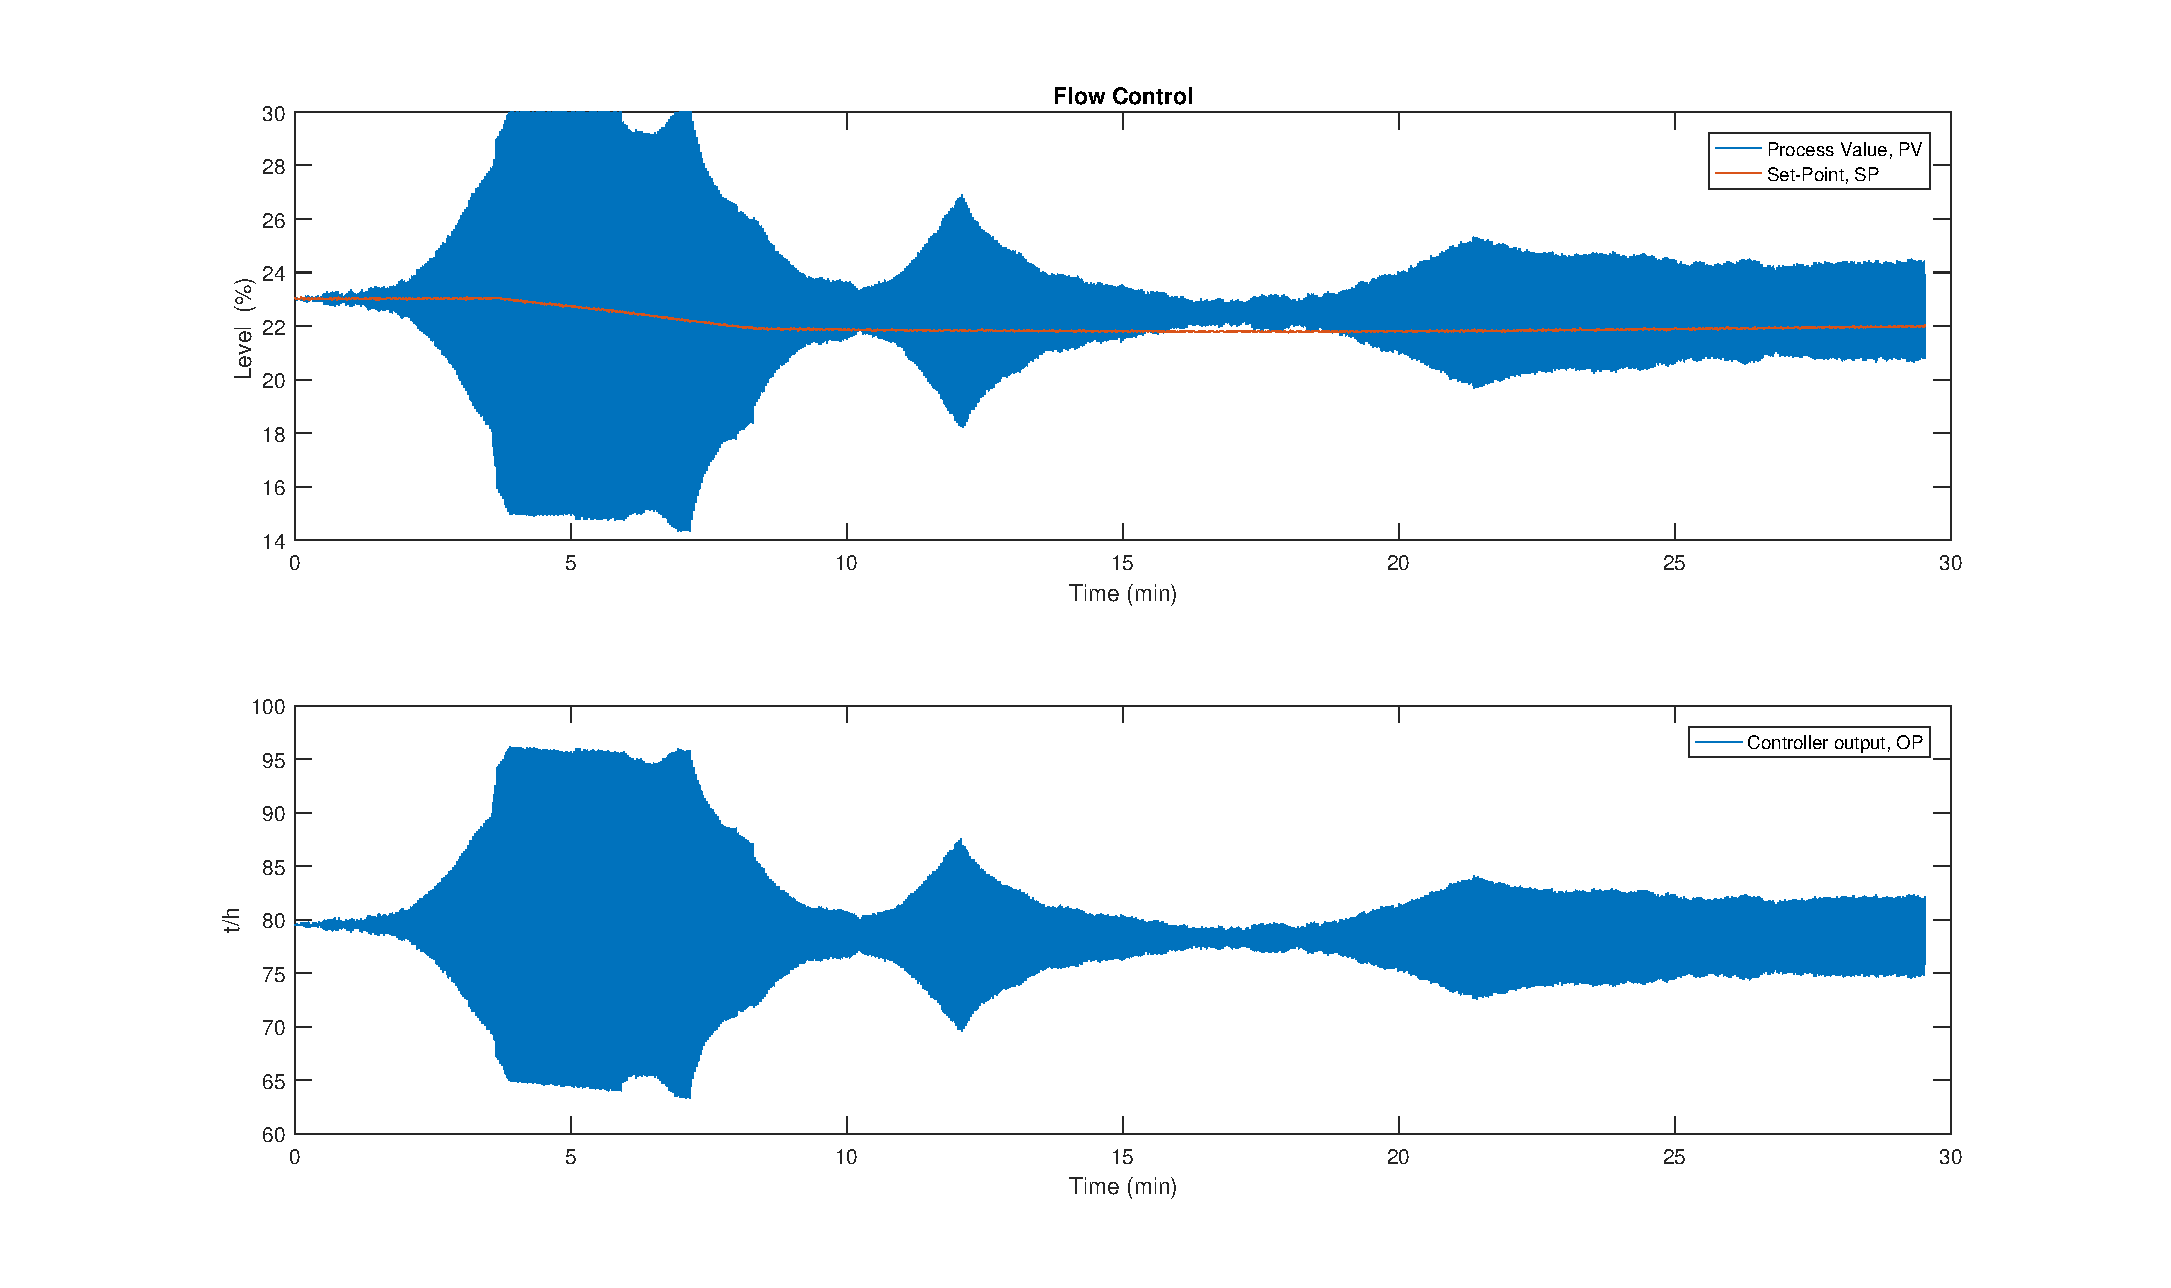
\includegraphics[width=0.85\textwidth]{fig/tuning/FC1019_critical.eps}
	\caption{Oscillations of the flow controller \texttt{24\_FC1019} with $K_{p_k} = 0.605$ from about $\SI{22}{\minute}$}
	\label{fig:fc1019_oscillations}
\end{figure}

\begin{figure}[ht!]
	\centering
	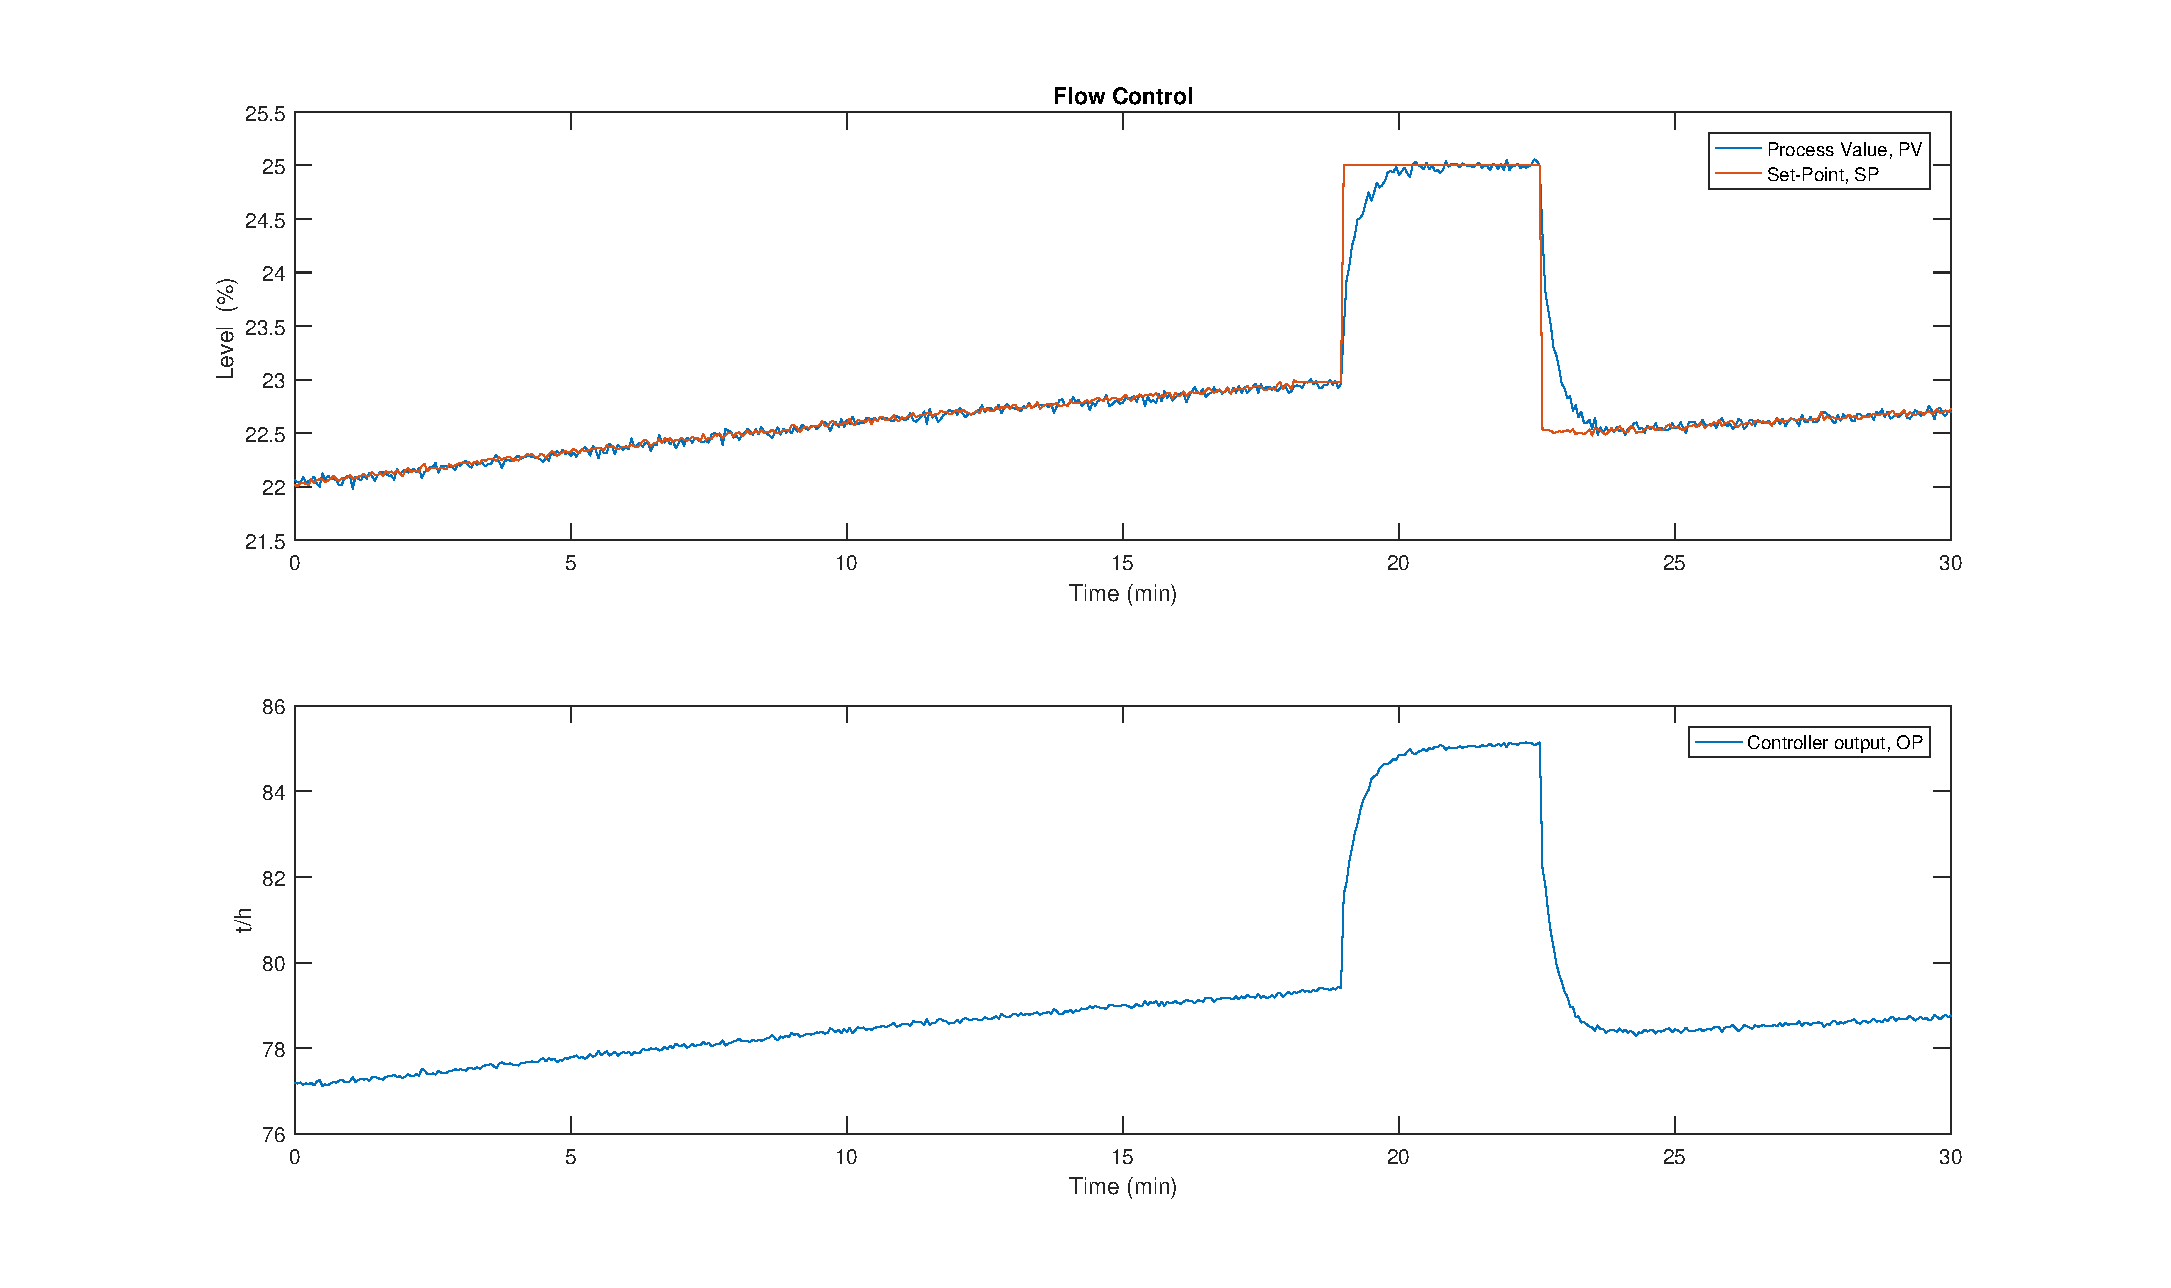
\includegraphics[width=0.85\textwidth]{fig/tuning/FC1019_tuned.eps}
	\caption{Response of \texttt{24\_FC1019} tuned using Ziegler-Nichols method}
	\label{fig:fc1019_tuned}
\end{figure}

\subsection{Tuning of \texttt{24\_FC1005}}
We now tune the controller \texttt{24\_FC1005}, another flow controller, this one controlling $D$, the distillate flow of Iso-butane. Using the same method as in the tuning of \texttt{24\_FC1019}, we find the critical values $K_{p_k} = 2.625$ and $T_k = 6 \si{\second}$. This yields the parameters $K_p = 1.18125$ and $T_i = 5 \si{\second}$. As we see in \autoref{fig:fc1005_tuned}, the we get a slow oscillation when switching back to external reference, but this is due to oscillations in the set point, and not the process value. We see that the process nicely follows the reference with high accuracy.

\begin{figure}[ht!]
	\centering
	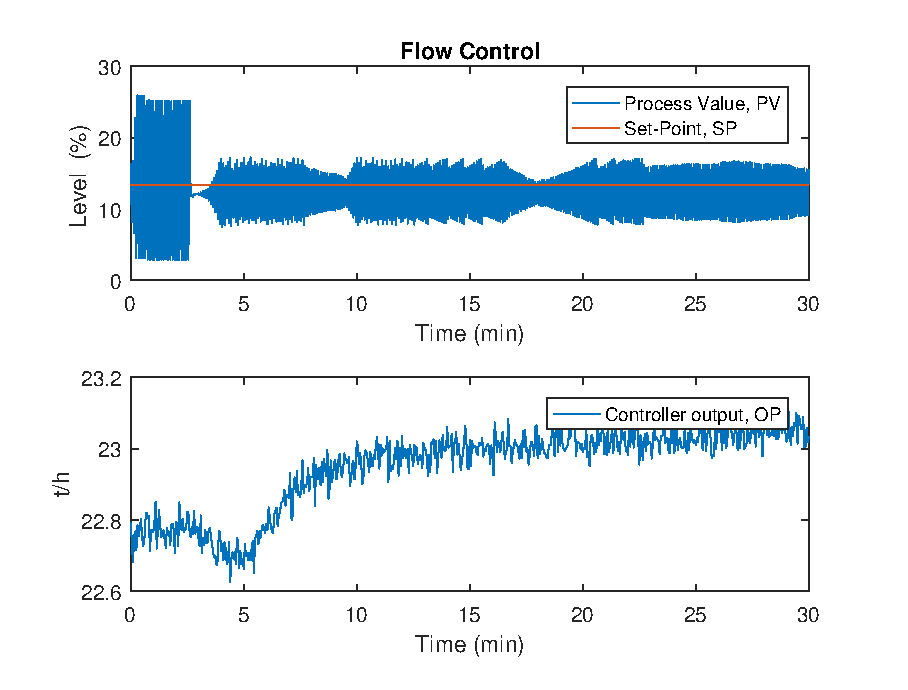
\includegraphics[width=0.85\textwidth]{fig/tuning/FC1005_critical.eps}
	\caption{Oscillations of the flow controller \texttt{24\_FC1005} with critical gain $K_{p_k} = 2.625$ from about $\SI{23}{\min}$}
	\label{fig:fc1005_oscillations}
\end{figure}

\begin{figure}[ht!]
	\centering
	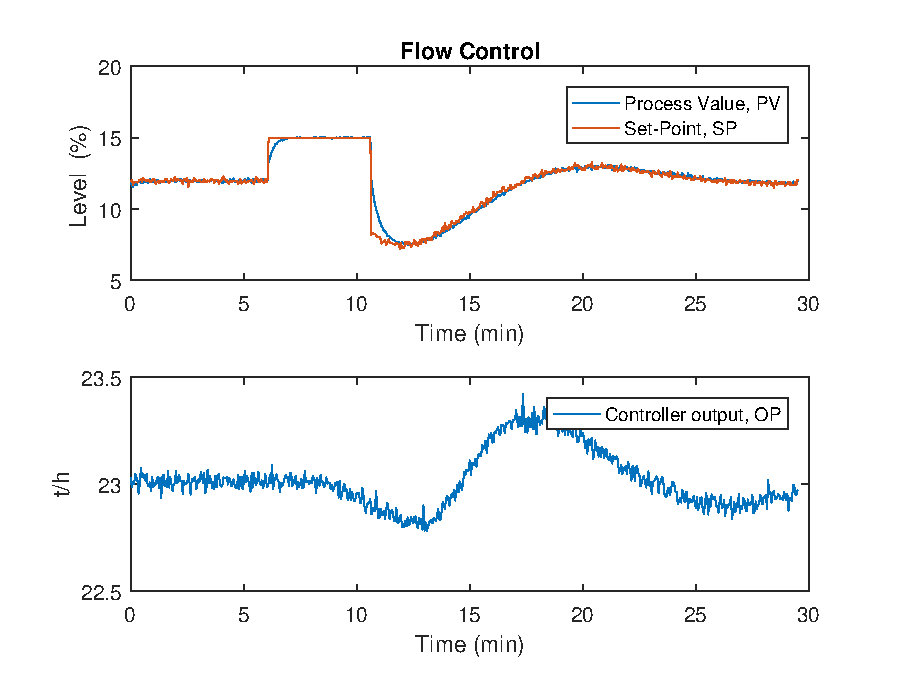
\includegraphics[width=0.85\textwidth]{fig/tuning/FC1005_tuned.eps}
	\caption{Response of \texttt{FC\_1005} tuned using Ziegler-Nichols method}
	\label{fig:fc1005_tuned}
\end{figure}

\subsection{Tuning of \texttt{24\_LC1028}}
Further we tune the level controller \texttt{24\_LC1028} wich controls the area for heat exhange in the bottom heat exchanger. This makes it indirectly control the bottom vapour flowrate $V$. Here we use the SIMC-method for tuning of PI(D)-controllers. Using this method we now need to take into account the internal scaling in the controller. By setting the integral time $T_i \to\infty$ we get a simple P-controller which we apply a step in the reference. By using the SIMC-tuning rules from \cite{skogestad2005multivariable} applied on a integrating step response we get

\begin{equation}\label{eq:simc}
	\begin{aligned}
		k' &= \frac{\Delta y}{\Delta t \Delta u}\\
		K_c &= \frac{1}{k'}\frac{1}{\tau_c + \theta} \\
		T_i &= 4(\tau_c + \theta)
	\end{aligned}
\end{equation}

where $\tau_c$ is chosen as $3\theta$ to achieve robustness. Smaller $\tau_c$ improves preformance, but makes the system less robust, as described in \cite{skogestad2005multivariable}. By measuring on \autoref{fig:lc1028_simc} we get the observations

\begin{equation}
	\begin{aligned}
		\Delta u &= 1\\
		\Delta y &= -0.3413\\
		\Delta t &= 462 \\
		\theta &= 8\\
	\end{aligned}
\end{equation}
which again gives the results

\begin{equation}
	\begin{aligned}
		K_c &= -42.3\\
		T_i &= 128\\
	\end{aligned}
\end{equation}

The scaling factor can be calculated as shown in \eqref{eq:scaling}, and when applying a step input with $\Delta y_{\text{ref}} = 2$, we get the immediate response $\Delta u_{\text{meas}} = -17.68$. $\Delta u_\text{exp} = K_p\Delta y_{\text{ref}} = 20$, which gives the scaling factor
\begin{equation}
	G = \frac{u_{\text{exp}}}{u_{\text{meas}}} = -1.13
\end{equation}
which again gives the controller parameters

\begin{equation}
	\begin{aligned}
		K_{p,\text{applied}} &= GK_c = 47.9\\
		T_i &= 128
	\end{aligned}
\end{equation}

This again leads to fairly good response, although the controller is maybe slightly aggressive. This is shown in \autoref{fig:lc1028_tuned}. The equations for the scaling parameter are given as

\begin{equation}\label{eq:scaling}
	\begin{aligned}
		\Delta u_{\text{exp}} &= K_p \Delta y_{\text{ref}} \\
		G &= \frac{\Delta u_{\text{exp}}}{\Delta u_{\text{meas}}} \\
		\implies K_{p,\text{applied}} &= GK_p
	\end{aligned}
\end{equation}


\begin{figure}[ht!]
	\centering
	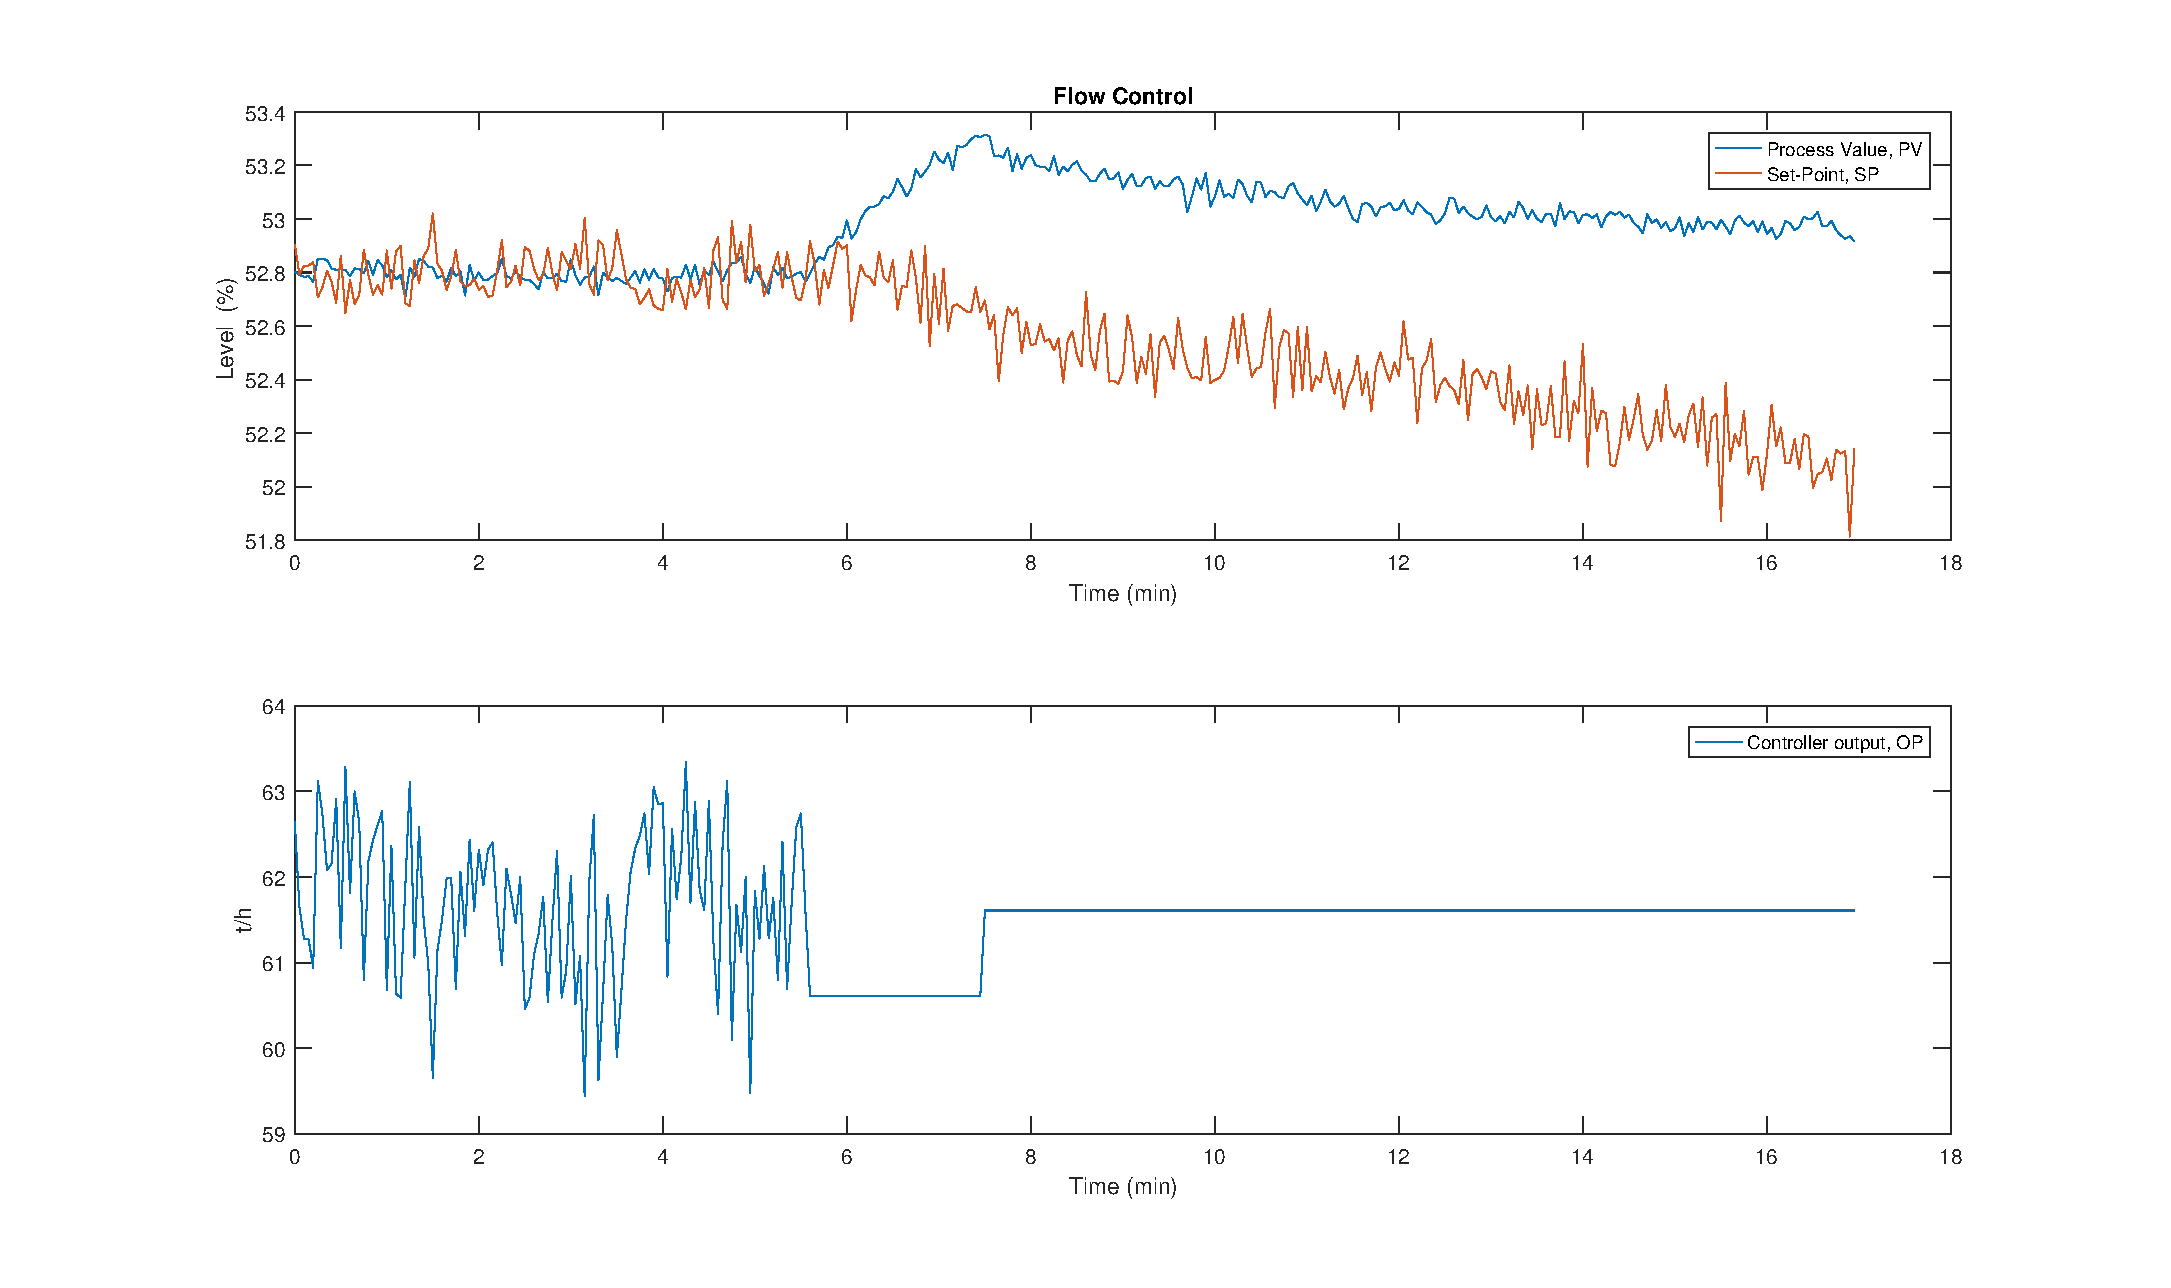
\includegraphics[width=0.85\textwidth]{fig/tuning/LC1028_simc.eps}
	\caption{Output of \texttt{24\_LC1028} with simple P-controller and applied step at $t \approx \SI{7}{\minute}$}
	\label{fig:lc1028_simc}
\end{figure}

\begin{figure}[ht!]
	\centering
	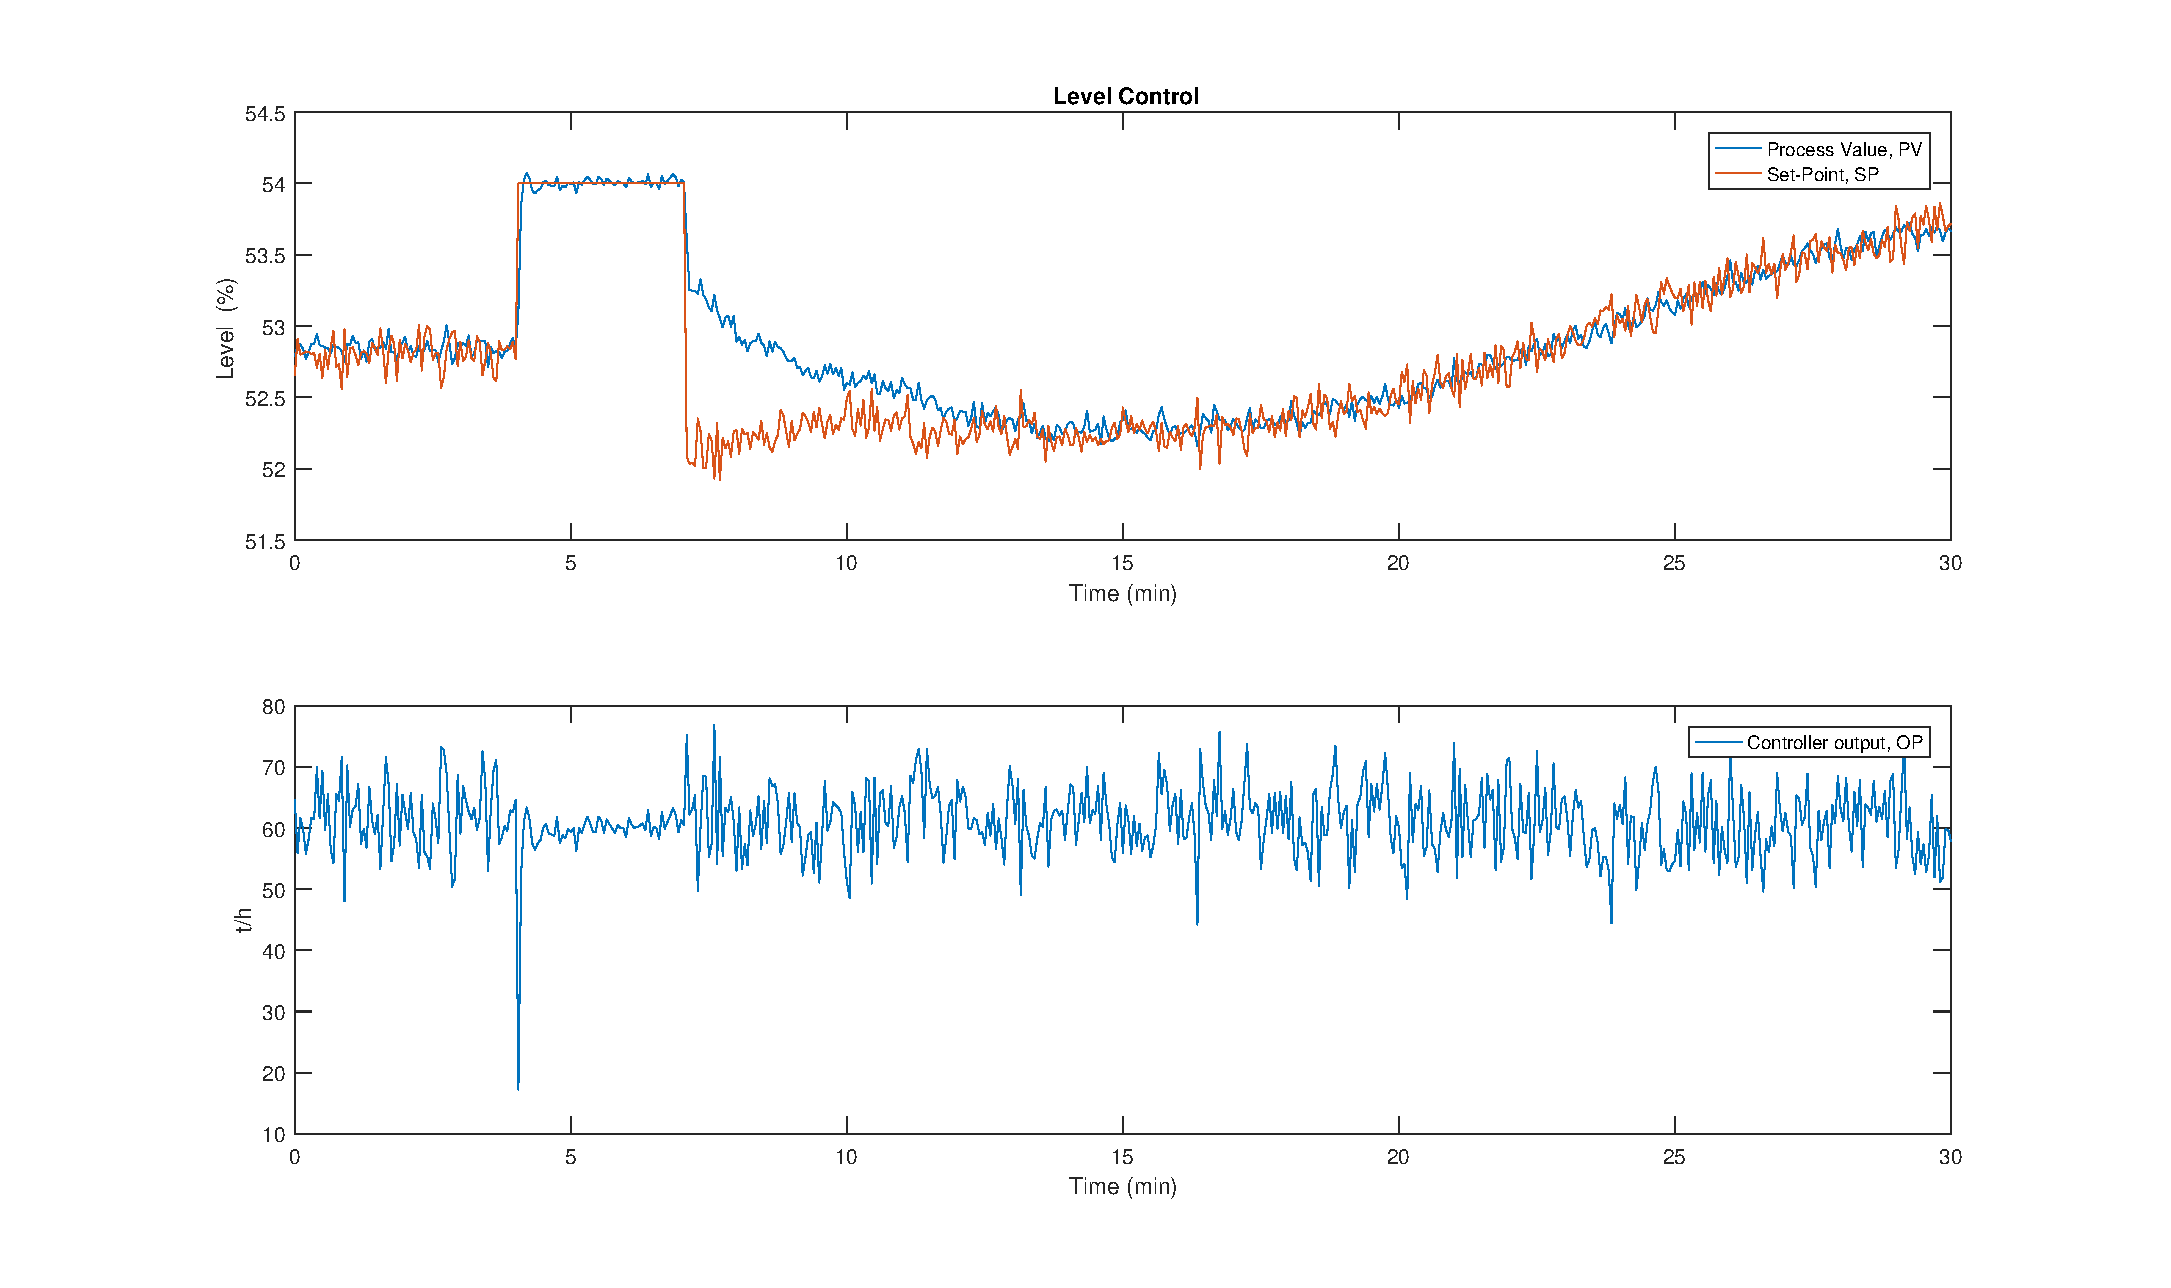
\includegraphics[width=0.85\textwidth]{fig/tuning/LC1028_tuned.eps}
	\caption{Output of \texttt{24\_LC1028} tuned using SIMC and PID-scaling}
	\label{fig:lc1028_tuned}
\end{figure}


\subsection{Tuning of \texttt{PC\_1024}}
When applying a step oon the input of the pressure controller \texttt{PC\_1024} we get the output response shown in \autoref{fig:pc1024_simc}. When then applying the SIMC method to this output response, we see that we do not have a proper first order model with delay or a clean integrating response with delay, we instead treat the time from the step until the integration starts properly as the time delay $\theta$. We also calculate the internal gain as in \eqref{eq:scaling} and obtain the parameters $G = -1.62$, $\delta u = 0.3$, $\delta t = 900$, $\delta y = -0.021$ and $\theta = 300$. Using the rules from \eqref{eq:simc} and chosing $\tau_c = \theta$ for faster control we get the controller parameters

\begin{equation}
	\begin{aligned}
		K_p &= GK_c = 17.5\\
		T_i &= 4(\tau_c + \theta) = 2400
	\end{aligned}
\end{equation}
This integral time seems quite large, but when looking at the response of the \texttt{PC\_1024} after tuning the parameters, shown in \autoref{fig:pc1024_tuned}, we see that the controller response is fairly good, and keeps the pressure well within acceptable deviations.

\begin{figure}[ht!]
	\centering
	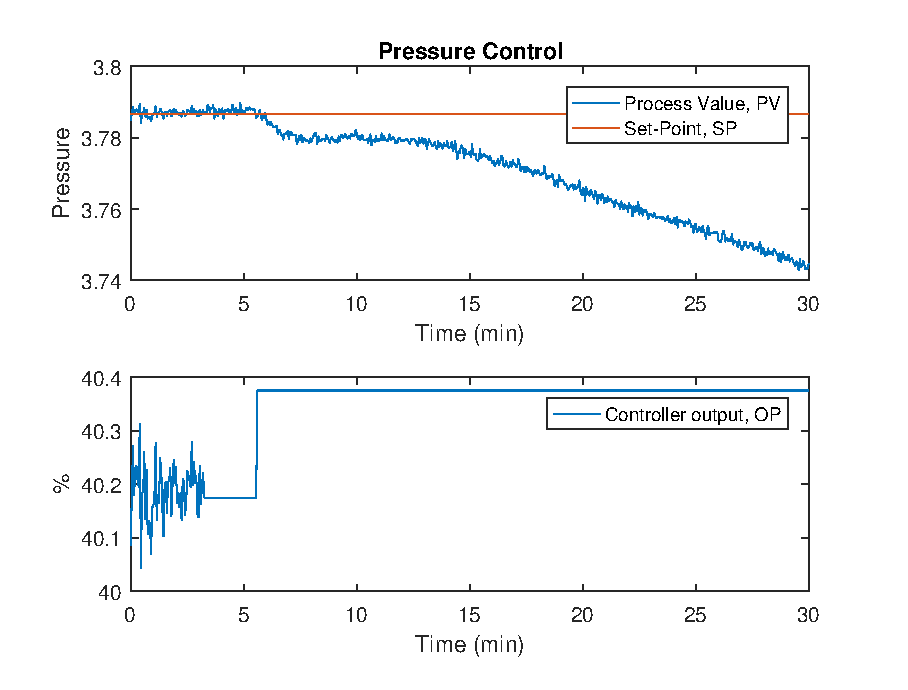
\includegraphics[width=0.85\textwidth]{fig/tuning/PC1024_simc.eps}
	\caption{Response of the controller \texttt{PC\_1024} when applying a step on input}
	\label{fig:pc1024_simc}
\end{figure}
\begin{figure}[ht!]
	\centering
	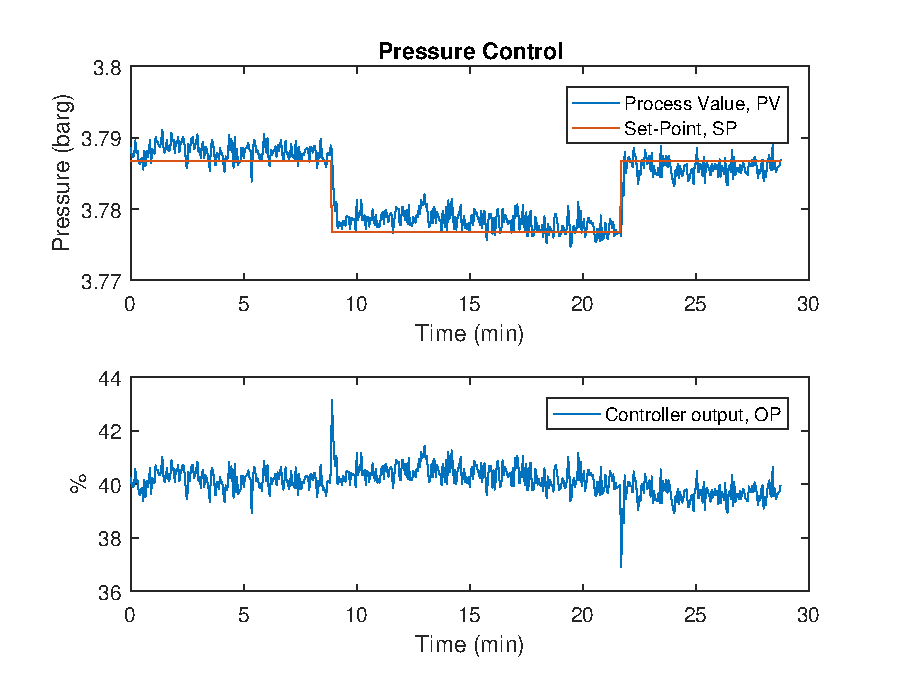
\includegraphics[width=0.85\textwidth]{fig/tuning/PC1024_tuned.eps}
	\caption{Response of the pressure controller \texttt{PC\_1024} after tuning and applying a step in the reference value}
	\label{fig:pc1024_tuned}
\end{figure}

\subsection{Tuning of \texttt{24\_FC1015}}
When it came to the controller \texttt{24\_FC1015}, I came to the conclusion that all responses were unstable when trying to use the classic tuning methods. I therefore went back to the even more classic method of trial and error. By tweaking $K_p$ and $T_i$ within reasonable limits we hit a set of parameters, $K_p = 0.2$ and $T_i = 5$, which gave fairly good response. This is shown in \autoref{fig:fc1015_tuned}. We see that the process value follows the reference pretty good.

\begin{figure}[ht!]
	\centering
	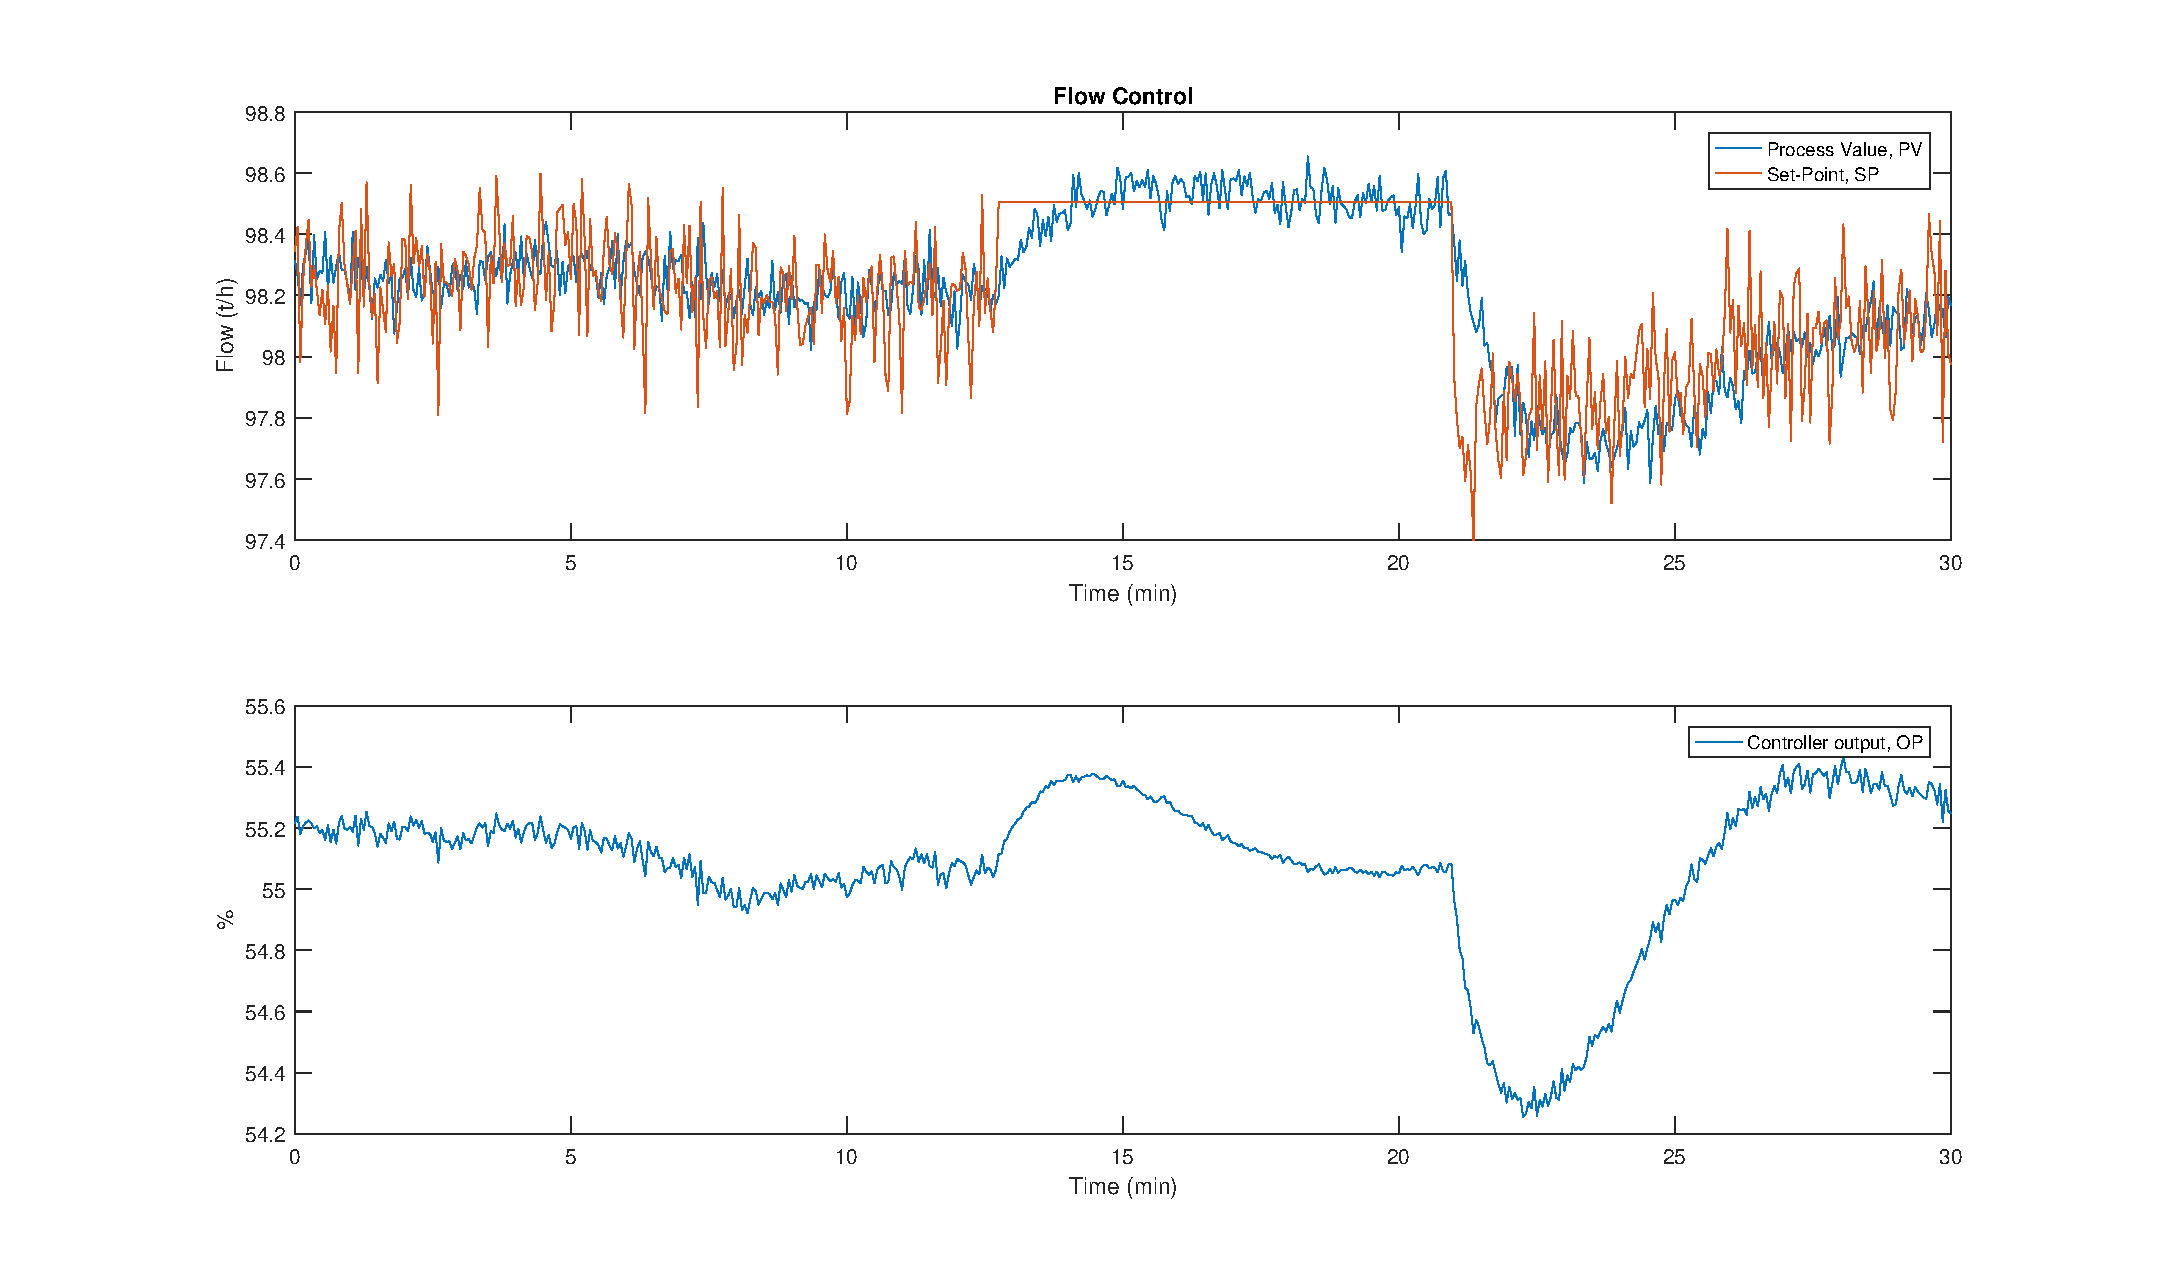
\includegraphics[width=0.85\textwidth]{fig/tuning/FC1015_tuned.eps}
	\caption{Response of the controller \texttt{24\_FC1015} after tuning using trial and error}
	\label{fig:fc1015_tuned}
\end{figure}

\section{Tuning and identification of level controllers}
We now move on to the identification and tuning of the level controllers \texttt{24\_LC1015} and \texttt{24\_LC1016}. These controllers